\documentclass[tikz,border=12pt]{standalone}
\usepackage[T1]{fontenc}
\usepackage{mathpazo}
\usepackage{amsmath,amssymb}
\usetikzlibrary{arrows.meta, positioning, calc, angles, quotes}

\definecolor{stblue}{HTML}{7B97AD}
\definecolor{rwgold}{HTML}{B8995E}
\definecolor{sage}{HTML}{7A9A7E}
\definecolor{dkbrown}{HTML}{3D3530}
\definecolor{wmgray}{HTML}{7B7067}
\definecolor{cream}{HTML}{F9F6F0}
\definecolor{border}{HTML}{D4C9B8}
\definecolor{terracotta}{HTML}{C47A6A}
\definecolor{lavender}{HTML}{907EA0}

\begin{document}
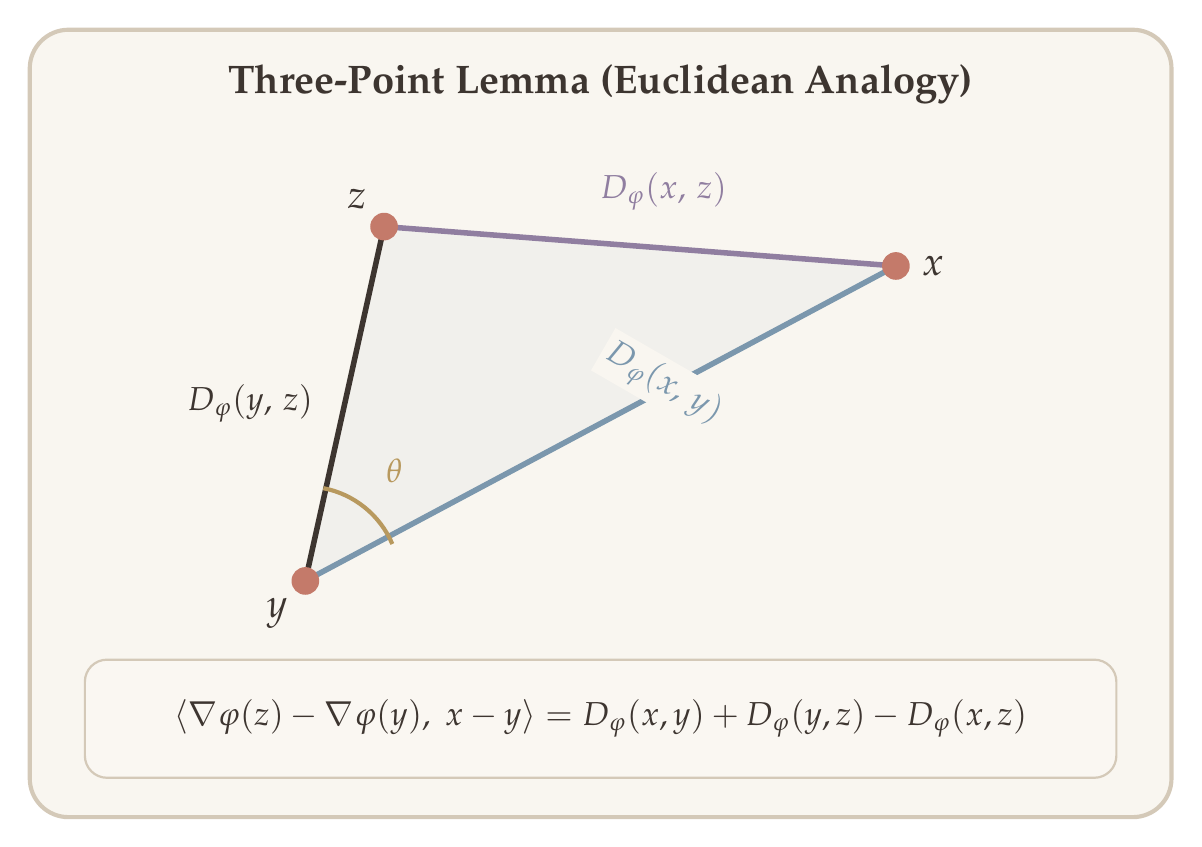
\begin{tikzpicture}[>={Stealth[length=4mm, width=3mm]}]

% Background
\fill[cream, rounded corners=14pt] (-0.5,-0.5) rectangle (14,9.5);
\draw[border, line width=1.5pt, rounded corners=14pt] (-0.5,-0.5) rectangle (14,9.5);

% Title
\node[text=dkbrown, font=\Large\bfseries] at (6.75,8.8)
  {Three-Point Lemma (Euclidean Analogy)};

% Triangle vertices
\coordinate (X) at (10.5,6.5);
\coordinate (Y) at (3.0,2.5);
\coordinate (Z) at (4.0,7.0);

% Fill triangle lightly
\fill[stblue, opacity=0.06] (X) -- (Y) -- (Z) -- cycle;

% Triangle edges with colored labels
\draw[stblue, line width=2pt] (X) -- (Y);
\draw[dkbrown, line width=2pt] (Y) -- (Z);
\draw[lavender, line width=2pt] (Z) -- (X);

% Edge labels — placed outside the triangle for clarity
\node[text=stblue, font=\large, fill=cream, inner sep=2pt, rotate=-30]
  at ($(X)!0.5!(Y) + (0.8,0.5)$) {$D_\varphi(x,\, y)$};
\node[text=dkbrown, font=\large, fill=cream, inner sep=2pt]
  at ($(Y)!0.5!(Z) + (-1.2,0.0)$) {$D_\varphi(y,\, z)$};
\node[text=lavender, font=\large, fill=cream, inner sep=2pt]
  at ($(Z)!0.5!(X) + (0.3,0.7)$) {$D_\varphi(x,\, z)$};

% Vertex labels
\fill[terracotta] (X) circle (5pt);
\node[text=dkbrown, font=\Large\bfseries, right=6pt] at (X) {$x$};
\fill[terracotta] (Y) circle (5pt);
\node[text=dkbrown, font=\Large\bfseries, below left=4pt] at (Y) {$y$};
\fill[terracotta] (Z) circle (5pt);
\node[text=dkbrown, font=\Large\bfseries, above left=4pt] at (Z) {$z$};

% Angle arc at y
\draw[rwgold, line width=1.5pt] (Y) ++(23:1.2) arc (23:79:1.2);
\node[text=rwgold, font=\large] at ($(Y) + (51:1.8)$) {$\theta$};

% Formula box
\fill[cream!90!white, rounded corners=8pt] (0.2,0.0) rectangle (13.3,1.5);
\draw[border, line width=0.8pt, rounded corners=8pt] (0.2,0.0) rectangle (13.3,1.5);
\node[text=dkbrown, font=\large] at (6.75,0.75)
  {$\langle \nabla\varphi(z) - \nabla\varphi(y),\; x - y \rangle
   = D_\varphi(x,y) + D_\varphi(y,z) - D_\varphi(x,z)$};

\end{tikzpicture}
\end{document}
